%        File: additional_info.tex
%     Created: Fri Jul 19 04:00 PM 2013 C
% Last Change: Fri Jul 19 04:00 PM 2013 C
%
\documentclass[a4paper]{article}
\usepackage[]{amsmath}
\usepackage[detect-all]{siunitx}
\usepackage{textcomp}
\usepackage{booktabs}
\usepackage[affil-it]{authblk}
\usepackage[]{graphicx}

\begin{document}
\title{Performance and optimization of X-ray grating interferometry}
\author{Matteo Abis, Thomas Th\"uring and Marco Stampanoni}
\affil{ETH Z\"urich and Paul Scherrer Institut}
\renewcommand{\today}{}
\maketitle
\begin{abstract}
A theoretical description of the performance of a Talbot and Talbot-Lau
type interferometers is developed, providing a framework for the
optimization of the geometry for monochromatic and polychromatic
beams. Analytical formulas for the smallest
detectable refraction angle and the visibility of the setup are derived.
The polychromatic visibility of the interference fringes is particularly
relevant for the design of setups with conventional X-ray tubes, and it
is described in terms of the spectrum of the source and the type of
beam-splitter grating.
\end{abstract}
\section{Methods}
Grating interferometry (figure~\ref{interferometer}) is an imaging technique yielding complementary
signals from the interaction of X-rays with matter. Besides the absorption
image, a phase shift \cite{phase,phase2} and a scattering \cite{scattering} signal
can be simultaneously retrieved from the interference pattern.

This approach does not rely on a highly coherent source, thus it can be applied
to ordinary X-ray sources and not only to synchrotron facilities.

\begin{figure}[h]
    \centering
    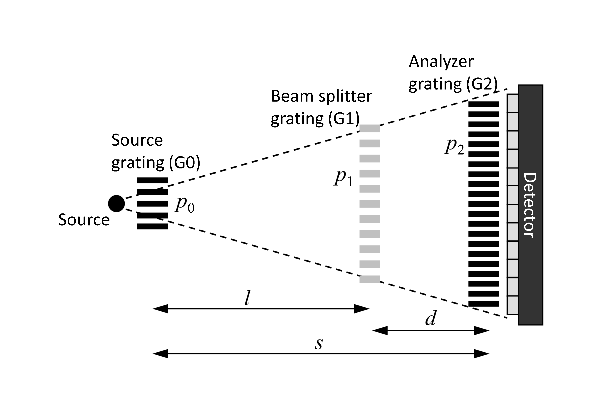
\includegraphics[width=0.5\textwidth]{grating_interferometer}
    \caption{Parameters of a grating interferometer. The Talbot
    interferometer does not include a source grating G0.}
    \label{interferometer}
\end{figure}

In order to achieve maximum performance, the design parameters of the
interferometer, such as the pitch of the gratings and their position have to
be tuned. Analytical formulas for a the smallest detectable refraction angle
and visibility are derived.

\section{New results}
The minimization of the smallest detectable refraction angle 
$\alpha_\text{min}$\cite{alphamin} for a Talbot intereferometer is achieved in two steps.
The smallest source sizes $w$ and analyser grating periods should be chosen,
according to the properties of the X-ray tube and the available grating
technology. Then, an optimum period $p_{11}$ of the beam-splitter grating can be
calculated as shown in figure~\ref{optimum_p1}.

\begin{figure}[h]
    \centering
    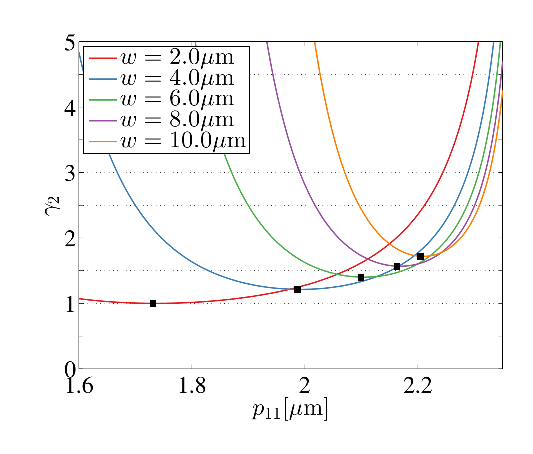
\includegraphics[width=0.5\textwidth]{optimum_p1}
    \caption{Optimization of a Talbot interferometer. The quantity
    $\gamma_2$ is proportional to the smallest detectable refraction angle
and it is shown that there is a minimum for different source sizes
$w$ and for $p_2 = \SI{2.4}{\micro\metre}$. The minima are the black
markers.}
    \label{optimum_p1}
\end{figure}

For the Talbot-Lau design, the smallest $\alpha_\text{min}$ is achieved for
the smallest sum of the pitches of G0 and G2, and is therefore limited by
the grating fabrication.

The duty cycle $\kappa$ of the absorption grating also affects the sensitivity of the
system, and it can be shown that, for an ideal grating, the optimum duty
cycle is $\kappa = 0.371$ in both configurations.

The dependence of the fringe
visibility on the photon energy is derived. The spectral acceptance of the
interferometer can then be analyzed as in figure~\ref{fringe_visibility}.
The numerical calculations show the visibility for a point source with a gaussian spectrum
at various Talbot orders and prove
that $\pi$-shifting phase gratings give better results than $\pi/2$ shifting
gratings, except for the first Talbot order, where they are substantially
equivalent. 

\begin{figure}[h]
    \centering
    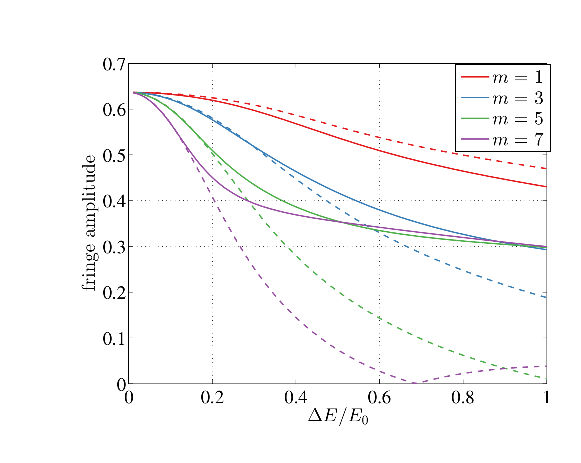
\includegraphics[width=0.5\textwidth]{polychromatic}
    \caption{Fringe visibility for a polychromatic beam of a point source as
    a function of the normalized energy bandwidth $\Delta E / E_0$ of a
gaussian spectrum for different talbot orders $m$ and for $\eta = 1$
(dashed lines) corresponding to a $\pi / 2$ shift in the phase grating
structures, compared to a $\pi$-shifting phase grating (solid lines).}
    \label{fringe_visibility}
\end{figure}

The results of these theoretical calculations have been used
in the design of a Talbot-Lau interferometer for a high-energy X-ray tube
(160 kVp) at the Paul Scherrer Institute (Switzerland).
An analysis of the performance and the first experimental results will be
presented.

\section{Submissions}
Part of the theoretical aspects in the present work are being submitted to
Phil. Trans. A.
Additionally, the presentation includes the experimental results from a new
interferometer designed according to these guidelines.

\begin{thebibliography}{9}

%\bibitem{edgeon}
%C. David and M. Stampanoni, \emph{A method for x-ray phase contrast
    %and dark-field imaging using an arrangement of gratings in planar
%geometry}, 
    %EP10167569.
\bibitem{phase}
C. David, B. N\"ohammer, H. Solak and E. Ziegler, Applied Physics Letters
\textbf{81}, 3287 (2002)
\bibitem{phase2}
A. Momose, S. Kawamoto, I. Koyama, Y. Hamaishi, K. Takai and Y. Suzuki,
Japanese Journal of Applied Physics
\textbf{42}, L886 (2003)
\bibitem{scattering}
F.Pfeiffer, T. Weitkampf, O. Bunk and C. David, Nature Physics
\textbf{2}, 258 (2006)
\bibitem{alphamin}
    T. Th\"uring, P. Modregger, S. H\"ammerle, S. Weiss, J. N\"esch and M.
    Stampanoni, AIP Conference Proceedings
\textbf{1466}, 293 (2012)
\end{thebibliography}
\end{document}


